% Indicate the main file. Must go at the beginning of the file.
% !TEX root = ../main.tex

%----------------------------------------------------------------------------------------
% CHAPTER 2
%----------------------------------------------------------------------------------------
\chapter{Theoretical Background} % Main chapter title
\label{Chapter2} % For referencing the chapter elsewhere, use \ref{Chapter1}
In this chapter, the relevant literature and background information is discussed.  
\section{Cellular Automata}
\subsection{An Overview}

CA are fascinating mathematical models, which typically have very simple rules that result in complicated behavior. They were first introduced by John Von Neuman \cite{sarkar2000brief} as models for self-replicating organisms. Since then they have found relevance in a wide variety of fields but are mainly used for modeling biological and physical systems. \\

Typically, CA are modeled on a discrete 1D or 2D lattice. The most famous CA are John Conway's Game of Life (GOL) and Steven Wolfram's Elementary CA, the former of which will be discussed in the below section.
\subsection{What is a CA?}

CA are some of the simplest computational models that exist. They consist of a discrete lattice or grid of cells (Typically these manifolds are 1D or 2D but can be $d$ dimensional). Each cell has a discrete state (or set of states). The most common of which, are binary states like in the case of Elementary CA and GOL \footnote{It is important to note, though, that variations of this exist and a lot of research has been done in the continuous state domain. A famous example of this within the artificial life (ALIFE) community is Lenia: Smooth life \cite{chan2018lenia}. The reason for this note is CA used for flood modeling as well as some other systems utilize this continuous state system}. Probably the most important aspect of CA systems are their local update rules'. In order for a cell to be updated, the cell considers the states of itself, as well as the states of its neighbors, and based on some predefined rule, the cell updates. In classical CA, cells update synchronously based on some global clock \footnote{This feature of classical CA also has variation, like in the case of stochastic CA \cite{fates2013stochastic}, where cells update asynchronously.}. Based on these features, very simple rules can result in extremely complex behaviour. Including Turing Completeness (like in the case of GOL and Rule 110) \\

To help build intuition about CA and its associated notation, I will discuss GOL.

\subsection{Mathematical Description of CA}
\subsubsection*{Definition}

An arbitrary CA is typically represented as a 4-tuple, with time, $T$, omitted:
\begin{equation} \label{eq:2.1}
	A = (L, S, N, f)
\end{equation}

Where $A$ is the CA; $L$ is the $d$-dimensional lattice; $S$ is the set of possible states; $N \subset L$ is the neighborhood; $f$ is the local update rule with $f: S^{N}\rightarrow S$. 
\subsubsection*{Defining Game Of Life}
The following are the general rules written in natural language and in the subsequent section we will demonstrate the notation used for such as system.

\begin{enumerate}[align=left]
	\item[Grid:] The Game of Life is represented as a two-dimensional grid of cells. Each cell can be either alive or dead, usually represented by binary values: 1 for alive and 0 for dead. The grid is typically depicted as a matrix-like structure.
	\item[Neighbourhood:] Each cell in the Game of Life has a neighborhood consisting of its eight adjacent cells, $\{-1, 0, 1\}^{2}$. This neighborhood is known as the Moore neighborhood. The state of a cell is influenced by the states of its neighboring cells according to the game's rules.
	\item[States:] In the Game of Life, each cell can be in one of two states: alive (1) or dead (0). This binary representation simplifies the rules and allows for the emergence of interesting patterns and behaviors.
	\item[Local Update Rule:] The evolution of the Game of Life is determined by a set of rules that dictate how cells change their states over time. These rules are applied simultaneously to all cells in the grid. The rules of the Game of Life are as follows:
	\begin{enumerate}
		\item Any live cell with fewer than two live neighbors dies, as if by under population.
		\item Any live cell with two or three live neighbors survives to the next generation.
		\item Any live cell with more than three live neighbors dies, as if by overpopulation.
		\item Any dead cell with exactly three live neighbors becomes alive, as if by reproduction.
	\end{enumerate}
\end{enumerate}
To describe GOL mathematically using the above rules we define $A_{GoL} = (L, S, N, \phi )$, where $L=Z^{2}$ is the two-dimensional discrete lattice, $S=\{ 0, 1 \}$ is the singular state set, and $N = \{ -1, 0, 1 \} ^{2}$ is the Moore neighborhood (or the eight surrounding neighborhood and itself). We say the neighborhood sum of some site $x$ is:
\begin{equation}
	S^{t}(x) = \sum_{n \in N}A^{t}(x+n)
\end{equation}
Every site is synchronously updated according to the local rule:
\begin{equation}
	A^{t+1} = \begin{cases}
		1 \text{ if } A^{t}(x) = 0 \text{ and } S^{t}(x) \in \{3 \} \\
		1 \text{ if } A^{t}(x) = 1 \text{ and } S^{t}(x) \in \{2, 3 \} \\
		0 \text{ otherwise }
	\end{cases}
\end{equation}
By applying these rules iteratively, the Game of Life evolves and creates various patterns, including static configurations, oscillators, and spaceships that move across the grid in an organized structure. The simplicity of these rules gives rise to complex and intriguing dynamics (see Fig \ref{fig:breeder}).

\begin{figure}[tbph]
	\centering
	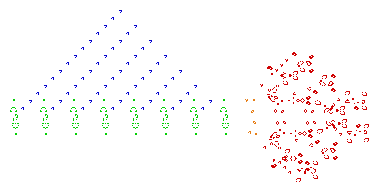
\includegraphics[width=0.8\linewidth, height=0.3\textheight]{Figures/Conways_game_of_life_breeder}
	\caption[Example Game Of Life Pattern (Breeder)]{The Breeder Pattern in Game of Life. Created by Hyperdeath - Own work, CC BY-SA 3.0, }
	\label{fig:breeder}
	\url{https://commons.wikimedia.org/w/index.php?curid=5117698}
\end{figure}


\subsection{Why are they useful?}
In the above section, although beautiful and impressive, the examples are not practical. But the same motivation and methods can be extrapolated to model physical or biological systems. For example, many differentiable equations that can be discretized in time and space can be modeled using CA. Many examples have been demonstrated over the years. In the following Chapter \ref{Chapter3}, the CADDIE model is discussed in detail. Other examples of practical CA include: particle simulation, chemical reactions, fire modeling, human and animal dynamics \cite{karafyllidis1997model, kier2005modeling, wolf2004lattice, alizadeh2011dynamic} to name a few.

\section{Deep Learning}
\subsection{What Is Deep Learning}
Deep learning (DL) is a subset of techniques within a class of algorithms known as Machine Learning (ML). In general, ML algorithms power increasingly more of our day to day lives \cite{lecun2015deep}. From auto-correct \cite{etoori2018automatic}, to search and recommendation systems \cite{haldar2019applying}, and even self-driving cars \cite{gupta2021deep}. The main difference between classical ML and DL is the former tends to require large amounts of domain knowledge and feature engineering to achieve good results \cite{dargan2020survey}. One of the main benefits of DL is their ability learn which features are important. However, classical ML tends to require a lot less data than DL models do. \\

 DL models are derived from simple neural networks (or multilayer perceptrons), which are motivated by biological neurons. They consist of a sequence of interconnected nodes, which creates a nonlinear mapping between inputs and outputs \cite{gardner1998artificial}. These nodes are connected by weights and signals are created via summing the inputs to the node and passed through an activation function making the system non-linear. By doing this, it is possible for the model to approximate complicated non-linear functions.
 
 \subsubsection*{Simple Multilayer Perceptron}
 
 \begin{figure}[h]
 	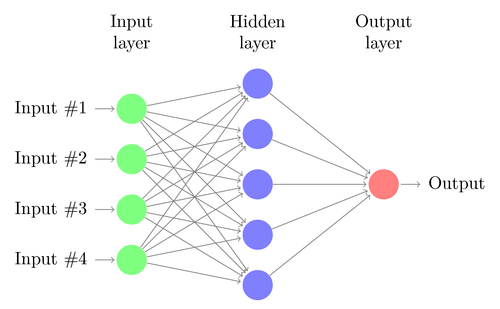
\includegraphics[width=0.75\textwidth]{../Figures/neural-network.png}
 	%	\centering
 	\caption[An ANN]{A simple depiction of an artificial neural network} \url{https://texample.net/tikz/examples/neural-network/}
 	\label{fig:appendix-mlp}
 \end{figure}
 
 \begin{equation*}
 	y =  \sigma\left(\sum WX + B\right)
 \end{equation*}
 Where
 \begin{align*}
 	y &  \text{ is the output or hidden layer} \\
 	\sigma &  \text{is the activation function} \\
 	X &  \text{ is the input vector} \\
 	W &  \text{ is the weight vector} \\
 	B &  \text{ Bias}
 \end{align*}
 Where Edges are weights and nodes are the sum of the weights *inputs + bias. An activation function like sigmoid or ReLu (which performs a kind of smooth mapping) is applied to this sum. What you might in the above equation is its similarity with the straight line function: $y = mx + c$. It indicates that a single neuron can learn to class a binary problem as long as it is linearly separable!. \\
 
 \subsubsection*{Categories of Deep Learning}
 There are three main categories of deep learning: Supervised learning, Unsupervised learning, and reinforcement learning. \cite{alzubaidi2021review}. And within these three categories there are many different techniques. This thesis only considers the convolutional neural network, which is a type of supervised learning technique / architecture. 

\subsection{Convolutional Neural Networks}
\subsubsection*{A Brief Overview}
A Convolutional Neural Network (CNN) is a type of Artificial Neural Network (ANN) that is commonly used in image and video recognition , natural language processing, and other tasks that involve processing input data with a grid-like structure \cite{li2021survey}. CNN's, like MLP's, are biologically motivated, however, CNN's can be said to mimic an animal's visual cortex \cite{angermueller2016deep}. They are  able to extract important spatial features such as edges and corners of images but are also able to extract extremely complex features \cite{KATTENBORN202124}. CNN's are much better at image-related tasks than MLP's. One of the greatest aspects of CNN's is the kernel. The same weights are applied to whole image. This greatly reduces the parameter count compared to MLP's where every input node is connected to every output node. This allows CNN's to be trained much faster than MLP's.

\subsubsection*{Common Components of a CNN Architecture} \label{CNN:components}
An example of a typical CNN architecture can be seen in figure \ref{CNN:components}
\begin{enumerate}[align=left]
	\item[Convolutional Layer:] This is what makes a CNN a CNN, this layer applies a set of filters to the input data to extract relevant features for the task at hand. The filters are typically small in size and designed to detect patterns, such as edges or corners. The output of the convolutional layer then goes through a non-linear activation function, such as the rectified linear unit (ReLU) \footnote{ReLU is generally the preferred activation function because it tends to allow for much faster training \cite{krizhevsky2017imagenet}}, which introduces non-linearity into the network.
	\item[Deepthwise Convolutional Layer:] This layer allows for feature mapping in singular channels. This makes it easier for the model to extract important features because it doesn't have to simultaneously learn all three channels (in the case of images) at once \cite{chollet2017xception}.
	\item[Pooling Layer:] This layer is meant to reduce parameter count and extract important features from the previous convolutional output. There are two types of common pooling layers: \begin{enumerate}
		\item[1:] Max Pooling. This applies a convolution that extracts the maximum value from the neighbourhood.
		\item[2:] Average Pooling. This applies a convolution and takes the average of the neighbourhood.
	\end{enumerate}
	\item[1x1 Convolutional layer:] This layer is very similar to a fully connected layer. It is used for dimensionality reduction or promotion. One can think of this as miniature neural network for each pixel \ element of the previous layers output. The output of a 1x1xD convolution will have the same spatial resolution as the input into this layer with D channels.
	\item[Fully Connected Layer:] This layer is just a typical MLP and is often used as the output layer for classification tasks. It works by connecting each element of the previous layer to each output node.
\end{enumerate}

\begin{figure}
	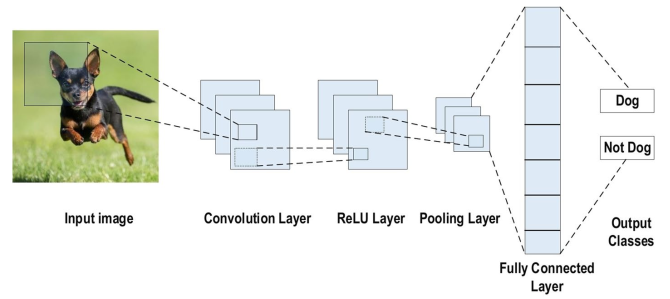
\includegraphics[width=0.75\textwidth]{../Figures/classical_cnn.png}
	\centering
	\caption[CNN]{A simple CNN architecture taken directly from the \citetitle{alzubaidi2021review} paper \cite{alzubaidi2021review}} 
	\label{simple_cnn}
\end{figure}

\subsubsection*{How Do CNN's Learn?}
The first step in order to train a CNN is to employ a loss function. There are many different types of loss functions that exist. Only loss functions used for regression tasks \footnote{A regression task involves predicting the actual values of interest apposed to a label like in classification tasks, which requires a different activation function in the output and a different loss functions.} will be mentioned due to the nature of this thesis. \\

The first is Mean Squared Error (MSE),

\begin{equation}
	\label{eq:2.2}
	MSE = \frac{1}{n}\sum_{i=1}^{n}\left(y_{i} - \hat{y}_{i}\right)^{2}
\end{equation}
The second is Mean Absolute Error (MAE),
\begin{equation}
	\label{eq:2.3}
	MAE = \frac{\sum_{i=1}^{n}\left|y_{i} - \hat{y}_{i}\right|}{n}
\end{equation}

Where $n$ is the number of samples; $y_{i}$ is the target value; $\hat{y}_{i}$ is the predicted value. \\

It is important to note that a loss function must be differentiable. The way neural networks are able to learn such complicated non-linear functions is because of the backpropagation algorithm. An optimizer algorithm like gradient descent (although many more exist) is used to minimize this loss function by driving it towards zero. It does this by calculating the optimizer with respect to the weight values for various inputs.

\section{The Relationship Between CA and CNN}
\label{ca-cnn}
\subsection{CNN as a CA}
As it turns out, CNN's are extremely similar to conventional CA \footnote{The idea for this section came from personal communication (Dr. Martin Schüle, May 2023)}. CA and CNN's are both types of mathematical models that can be used to process and analyze data with a grid-like structure, such as images or time series data. \cite{PhysRevE}

Both models operate by processing the input data in a local and hierarchical manner. In a CA, the state of each cell is updated based on the states of its neighboring cells. In the case of Wolfram's Elementary CA and GOL, this is done with a look-up table. CNN's use filters / kernels, which are applied to local patches of the input data to extract relevant features. However, one can think of a neighbourhood as a $NxM$ kernel or filter. In fact, by utilizing a cleverly constructed kernel and activation function, one can model many CA. A simple example of this would be game of life represented as a convolution. \\

A convolution is defined as: \\

\begin{equation*}
	g(x,y) = \omega f(x, y)
\end{equation*}
Where $f$ is the function to be convolved; $\omega$ is the kernel or filter; $g$ is the resulting convolution. For GOL we define the kernel as

\begin{gather*}
	\omega = 
	\begin{bmatrix}
		1 & 1 & 1 \\
		1 & 9 & 1 \\
		1 & 1 & 1
	\end{bmatrix}
\end{gather*}


And then add an activation function, $\sigma$: \\ \\

\begin{equation}
	\sigma(x, y) = \begin{cases}
		1, & \text{if } g(x, y) \in \{3, 11, 12\} \\
		0, & \text{else}
	\end{cases}
\end{equation}

Then the components of the 4-tuple (see Eq. \ref{eq:2}) becomes,
\begin{equation}
	\label{eq:2.4}
	A_{GOL} = (L, S, \ \omega , \ \sigma )
\end{equation}
It turns out that CNN's can learn the rules of arbitrary CA's \cite{PhysRevE}, for example GOL, and it doesn't need a particularly deep architecture to do so. it does this by essentially learning the kernel / filter weights that needs to be applied. To use a CNN as a CA (with a binary state space), you essentially turn the CA into a binary classification problem to predict the state of each cell.

\section{Neural Cellular Automata}

This section attempts to summarize the paper, \citetitle{growing_nca} by \citeauthor{growing_nca} \cite{growing_nca}
\subsection{Brief Background}

The motivation for this NCA, like the MLP and CNN, is biologically motivated. In this case, cell morphology was the topic of interest. How do cells, using local information like the cells around them and chemical gradients 'know' what type of organ or tissue to become? This incredible ability of living systems is known as self-organization. The goal of \citeauthor{growing_nca} was to determine cell-level rules which simulate the behavior of these biological systems, like creating complex shapes  starting from a single cell, maintaining that shape and regenerating itself once damaged. This is resistance to perturbation is a key difference between NCA and CA. Typical, deterministic CA are extremely sensitive to noise. A single cell state change may destroy the whole system and result in chaos, where NCA can learn to adapt.


\subsection{The Model}
Now that we have some basic foundational knowledge about CA and CNN's, we can move on to the real NCA (or differentiable, self-organizing systems). As discussed in section \ref{ca-cnn}, a CNN can be seen as a type of CA, but utilizing a continuous state-space instead of a discrete one. We can also increase the amount of channels each cell has to an arbitrary number. In the paper, they found 12 hidden states to be a good number. As can be seen in (fig \ref{fig:nca}), this model can be thought of as a “Recurrent, Residual Convolutional Network with ‘per-pixel’ Dropout”. The 'per-pixel dropout' refers to the stochastic updating of cells, where only a certain percentage of cells are updated to the next time step. We start from a single black pixel in the center of a blank image and run the model on it over a number of steps where the output of the model increments the input (i.e. recurrent).
\begin{figure}[h]
	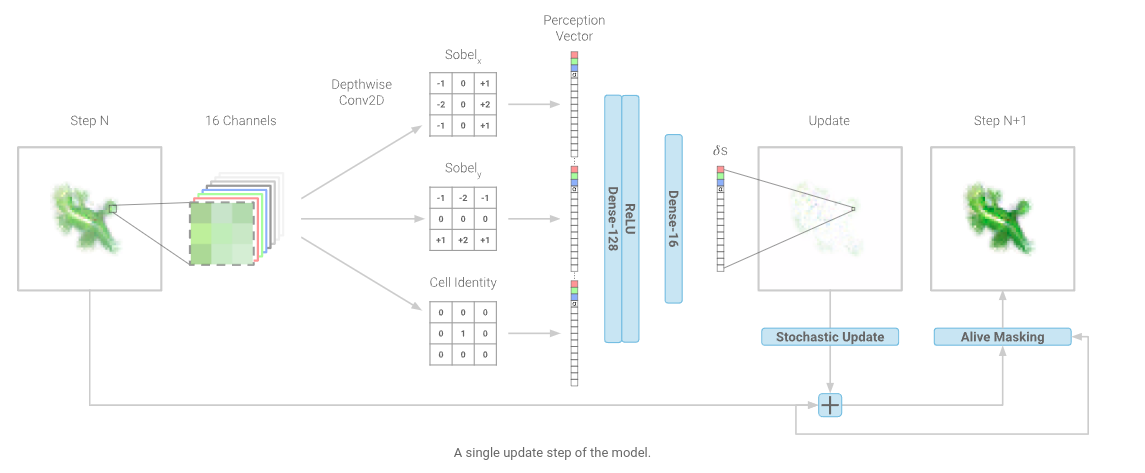
\includegraphics[width=1\textwidth]{../Figures/growing_nca.png}
	\centering
	\caption[NCA]{What a single step of the nca model looks like. This image is taken directly from the \citetitle{growing_nca} paper \cite{growing_nca}} 
	\label{fig:nca}
	\url{https://distill.pub/2020/growing-ca/}
\end{figure}

\subsection{Training} \footnote{The paper outlines multiple experiments. Only the initial experiment titled "Experiment 1: Learning to Grow " will be covered.}
We start from a single black pixel, iterate the model over $x$ time steps, then compare the final result of this model with the target image we are training the model. We then perform a per-pixel difference or MSE (equation \ref{eq:2.2}). Based on this loss, we use the ADAM optimizer to back-propagate through time and adjust the weights accordingly until the model learns to grow or morph into the target image (see Fig \ref{fig:nca-train}).
	
\begin{figure}[h]
	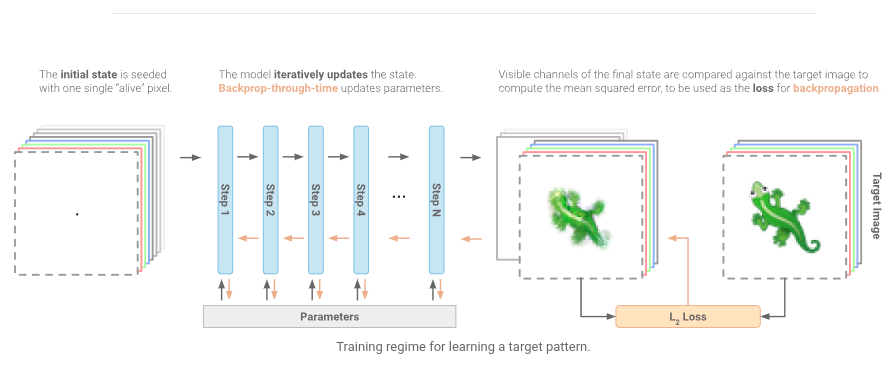
\includegraphics[width=1\textwidth]{../Figures/training_nca.png}
	\centering
	\caption[NCA Training]{How the model learns a target pattern. This image is taken directly the \citetitle{growing_nca} paper \cite{growing_nca}} 
	\label{fig:nca-train}
	\url{https://distill.pub/2020/growing-ca/}
\end{figure}

